\chapter{State of the art}\label{A:stateOfTheArt}

This chapter aims to provide a vision of how the audio-visual media production sector has been, and still is, converging to IP.

Moreover, this chapter will be focused on the topics related to media production over an IP environment and, specifically, the ones related on this thesis study and proposal. These are virtualization, monitoring and application core service.

Within the broadcast workflow two main scenarios can be distinguished: production and diffusion (i.e.: broadcasting). It is important to remark that this thesis is going to be focused only on the production scenario (i.e.: live production, see Figure \ref{F:bebooss}).

\section{Media content production}

This section summarises the standard formats currently used in audio-visual media content production and how they are adapted to reach IP convergence.

\subsection{Standard formats}

In production environment, broadcasters manage their audio and video content in an uncompressed or slightly compressed state. The main reason is to ensure they deliver the best quality possible (i.e.: lossless quality) of their digitized data. Besides, the goal to deliver best quality possible is also intended for diffusion environments but taking into account bandwidth usage constraints.

\subsubsection{Media formats in production environment}

In 1989, SMPTE (The Society of Motion Picture and Television Engineers \cite{smpte}) standardized a family of digital video and audio interfaces based on coaxial cable, called SDI (Serial Digital Interface \cite{SDI}), which is used for transport of uncompressed digital video and audio in a television studio environment. 

Around SDI there are other related standards which are focused in specific solutions (i.e.: to support higher video resolution, media qualities, media formats, frame rates, audio channels, synchronization,\ldots). An example is the HD-SDI \cite{SDI} standard (High-Definition Serial Digital Interface, defined in SMPTE 292M) which provides enough bandwidth to transport HD video fromats (i.e.: up to 1,485 Gbps). Other SDI related standards are the 3G-SDI \cite{3GSDI} and 12G UHD-SDI \cite{UHDSDI}, which give support to FHD (i.e.: Full HD, 1080p resolution up to 2,970 Gbps bitrates) and 4K (i.e.: UHD cinema resolution up to 12 Gbps bitrates) video formats, respectively. 

The main parameters related to uncompressed audio and video signals are:

- For video:
\begin{itemize}
\item Color depth: this is also referred to as bits-per-pixel (BPP), and defines how many colors can be represented by each pixel in the video frames (i.e.: still images). A number $\mathrm{n}$ of bits per pixel provides $\mathrm{2^{n}}$ colours per pixel.
\item Video resolution: this is measured by the number of pixels wide by the number of pixels high of a video stream.
\item Frame rate: this is the number of still images (i.e.: video frames) per second (i.e.: fps) sent as part of the video stream. 
\end{itemize}

Then, the bitrate generated by an uncompressed video stream can be calculated as:
\begin{equation}\label{E:videobitrate}
bitrate (bits/s) = color\ depth (bits/pixel) \cdot frame\ size (pixels/frame) \cdot frame\ rate (frames/s) 
\end{equation}

- For audio:
\begin{itemize}
\item Sample rate: This is the average number of audio samples obtained in one second and its measurement unit is hertz (Hz).
\item Bit depth: this is the number of bits an audio sample is recorded at.
\item Number of channels: this is the number of separate streams of the audio information.
\end{itemize}

Then, the bitrate generated by an uncompressed audio stream can be calculated as:
\begin{equation}\label{E:videobitrate}
bitrate (bits/s) = sample\ rate (samples/s) \cdot bit\ depth (bits/sample) \cdot channels  
\end{equation}

A typical HD-SDI stream with 10 bits per sample and YUV\footnote{In YUV, ‘Y’ represents the brightness, or luma value, and ‘UV’ represents the color, or chroma values (U is the blue-difference and V is the red-difference). In contrast, the values of the RGB encoding scheme represent the intensities of red, green and blue channels in each pixel. YUV is used because the human eye perceives chroma worse than luma, and therefore a chroma subsampling factor of 2 or 4 can be applied (i.e.: only half or a fourth of color samples are taken, compared with the luma or black-and-white signal.)} 4:2:2 color encoding scheme is applied with Y sampled at 74.25 Msamples per seconds and $\mathrm{C_{B}}$ (i.e.: U) and $\mathrm{C_{R}}$ (i.e.: V) sampled at 37.125 Msamples per seconds.  So, the amount of bandwidth accepted is:
\begin{equation}\label{E:sr}
10 bits/sample \cdot (74.25 Msamples/s + 2 \cdot 37.125 Msamples/s) = 1.485 Gbps
\end{equation}

This number includes both the active part of the image and the inactive part (synchronization).

If the visible part is calculated, a video sampled at 50 frames per second at interleaved frame rate, with frame size of 1920 x 1080 pixels and bit depth of YUV 4:2:2 fits inside HD-SDI:
\begin{equation}\label{E:srex}
25 \cdot 1920 \cdot 1080 \cdot 10 \cdot [1 + 0.5 + 0.5] = 1.036 Gbps
\end{equation}

\subsubsection{Media formats in diffusion environment}

The wide adoption of low-delay encoding (e.g.: JPEG2K, AVC, AVCi, VC-2) for high quality video streams could represent a new opportunity to reduce the bandwidth consumption in several scenarios (e.g.: diffusion). Likewise, high-compression mechanism as MPEG4 H264 or HEVC could be useful to transport media content through very limited network resources scenarios (as Internet or cloud-based systems).

Finally, to remark that lossless compression formats (e.g.: the lossless encoding profile of JPEG2K) are also considered for production environments.

\subsection{Convergence to IP}

This section focuses on IP convergence, from the transport and media types points of view, and describes how media content is transported in an IP environment over tools that are going to be developed during this thesis, to reach the goal of convergence of the media content production to IP. 

Since SDI standard was released, new encapsulation audio (i.e.: AES67-2013 \cite{AES}) and video (i.e.: SMPTE 2022-6 \cite{ST2022}) standards have appeared for the transport of high-quality media signals over IP Networks. Also, further specific solutions, such as managing packet loss recovery using FEC (SMPTE 2022-5 \cite{ST20225}), provide higher robustness.

In the middle of 2014, the Video Services Forum (VSF \cite{VSF}) has formed a new working group (SVIP \cite{SVIP}, which focuses on defining and researching requirements for video over IP without SDI encapsulation) looking at new encapsulation mechanisms for audio, video and ancillary data into IP without using SDI framing (raw data) to develop or recommend a standard for video over IP without SDI encapsulation.

Moreover, in 2013 SMPTE, VSF and EBU (European Broadcasting Union) created the JT-NM task force (JT-NM) to drive the broadcasting industry towards a full IP adoption by providing guidelines to enable a successful migration. Currently, the JT-NM is working to develop a reference architecture to help all involved layers to agree on all cross issues while defining specific requirements over concrete use cases to uncover missing definitions to address the general scenario \cite{jtnm}.

Both gropus aim to study and define the requirements for video over IP/Ethernet within plant (e.g.: video, audio, ancillary data, bundles, timing, sequencing and latency) in order to research over current and proposed solutions so that to report on gaps between requirements and existing solutions (especially regarding existing SMPTE 2022 Standards) and finally to propose scope for follow on activity, if required.

\subsubsection{Layer 2 - Data Link}

Besides, it is important to remark the role of the Ethernet \cite{eth} protocol, which was standardised in 1983 and since then it has been increasing its speed rate from the initial 10 Mbps to 100 Gbps (foreseen 400 Gbps by IEEE P802.3bs \cite{ethbs} Task Force), with currently easily affordable 10 Gbps and 40 Gbps interfaces. These rates are enough to accommodate current broadcast formats (e.g.: HD-SDI at ~1.5 Gbps, 3G-SDI at ~3 Gbps and UHD at ~12 Gbps) and future formats, thanks to the nature of the packet technologies that make them completely agnostic to the upper formats and indeed transparent for future formats in contrast with current media transport technologies which are completely bounded with the transported formats (i.e.: standard cable video formats used over broadcast environments). On the other hand, Ethernet does not have any timing awareness or QoS assurance, and therefore it is difficult to accommodate current broadcast requirements over this technology. Since Ethernet is widely used in the IT industry as COTS\footnote{COTS refers to products that are commercially available and can be bought ready to use. The use of COTS products/services may imply a reduction of overall development, deployment and maintenance time and cost} (Commercial Off-The-Shelf) switches, the next logical step is to use this technology in the broadcast industry deployments and assess specific necessary features as the latency deviation or packet loss.

To address some of the inherent Ethernet limitations, Audio Video Bridging (AVB, IEEE 802.1BA-2011 standard \cite{avb}) appeared in 2011. AVB is a set of standard extensions to the Ethernet IEEE 802.1 \cite{8021} focusing on timing and QoS guarantees within local area networks. Its approach is a plug-and-play platform to ease transition from current transport technologies to the newer ones using the same workflows, but the current version is still limited to local premises and limited topologies. Since November 2012, because more varied industry sectors joined the task group, a more general name, the Time Sensitive Networking (TSN task group \cite{tsn}), was created to carry on with the new developments.

A new paradigm, the SDN (Software-Defined Networking) is emerging \cite{sdn}. SDN separates the control and forwarding plane besides creating northbound interfaces to interact with external applications, enables new flexible and customised network operations and deployments. There are a lot of foreseen benefits from this approach but to be fully capable of supporting all type of streams some extensions should appear, such as the specific extension which has been released by the ONF (Open Networking Forum) to address timing restrictions \cite{sdn}.

Related to the above statements, the recent advances in chip designs by industry leaders (such as Intel, Broadcom, Xilinx and Altera) have eased a strong movement towards consolidation of complex functions (e.g.: encoding, transcoding, conversion) into a single device, instead several disparate platforms. Additionally, these hardware advances imply the chance of using software-centric frameworks, which provide for greater flexibility and customization from a business standpoint. Both advances are enabling a broader adoption of upcoming media technologies at a reduced cost, without compromise on quality, flexibility nor capability. 

\subsubsection{Layer 3 - Network}

IP is the de facto standard and within its protocol suite there are some solutions which help to transport media content efficiently. For instance, IP supports the multicast \cite{mc} paradigm operation using widely supported routing protocols (e.g.: IGMP), but the computational and scalable complexity of these protocols tends to difficult and limit deployments.

In terms of QoS, IP has a field known as ToS/DSCP \cite{tosdscp} which marks the header packets along their way to help mappings with lower-layer protocols (e.g.: Ethernet or MPLS) to implement QoS at the buffer level.

\subsubsection{Layer 4 - Transport}

UDP has been preferred over TCP for real-time transport because of its connectionless nature and avoidance of unnecessary retransmission and congestion avoidance techniques for live streams. RTP (Real Time Protocol), whose most deployed version is RFC 3550, was initially introduced to audio and video services, to add supplementary data fiels in order to enhance the UDP protocol (i.e.: timestamp field, sequence number, payload identification), together with the protocol for control purposes (i.e.: RTCP, which stands for Real Time Control Protocol). RTCP takes care of monitoring the QoS of the audiovisual transmission. Recently, new extensions have appeared introducing new header options to support the adoption of services related to media production workflows. Specifically, RTP and RTCP extension have been proposed to accommodate media specific info over IP.

\subsubsection{Signaling and metadata}

In the signaling layer, protocols such as RTSP (Real Time Streaming Protocol) for end-to-end session control or SDP for service description provide capabilities for the stream management. Furthermore, media wrappers aim to gather different types of programme media and associated information, as well as generically identify this information. Different media wrapper formats are in use at this time, but, for the media industry, it is important that the wrappers have characteristics like openness, extensibility and performance. The MXF (Material Exchange Format) is a container format \cite{mxf}, which supports a number of different streams of coded based by enabling interoperability between different platforms. This is done by encoding in any type of video and audio compression formats, together with a metadata wrapper which describes the material contained within the MXF file. 

\section{Migration to cloud}

This section is related to the previous one but focusing on how OTT\footnote{OTT refers to the service you use over the network services of your service provider. An example of OTT service is Youtube, which lets you playback video content on top of the infrastructure of several ISPs (Internet Service Providers).} \cite{ottVSiptv} content technologies (i.e.: video delivery techniques) are giving new chances to enhance audio-visual media production to IP convergence, concretely within the cloud computing concept. 

\subsection{Cloud computing}

Cloud computing describes the delivery of shared computing resources (software and/or data) on demand through the Internet. Cloud computing is defined by the NIST recommendations \cite{nistcc}. So, for many reasons like flexibility, scalability, security, data protection, agility and cost many organisations are migrating to cloud computing environments. 

Nowadays, cloud computing defines three fundamental models named SaaS, PaaS and IaaS, as seen in Figure \ref{F:cloudComputingLayers}, that are organized through application/service, platform and infrastructure layers.

\begin{figure}[htb]
\begin{center}
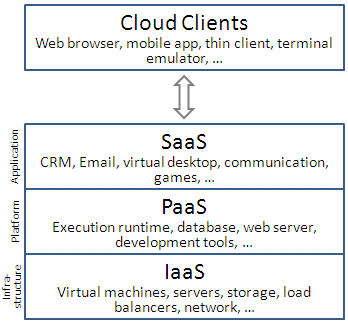
\includegraphics[width=0.6\textwidth]{./images/Cloud_computing_layers.png}
\caption{Cloud computing layers}
\label{F:cloudComputingLayers}
\end{center}
\end{figure}

Moreover, there are different deployment models depending on the product to be delivered (e.g.: specific service or application), which are related to the resources from the entity that is offering or using such product. The main deployment models are:

\begin{itemize}
\item Public: when applications/services run over resources that are open for public use, which may be free. The fact of being public/opened implies much more complexity in terms of security issues.
\item Private: when infrastructure is operated solely for a single organization, whether managed internally or by a third-party, and hosted either internally or externally. This cloud type might be similar in terms of architecture design from the public one.
\item Hybrid: when a composition of two or more clouds (private or public ones) are treated as distinct entities but are bound together, offering the benefits of multiple deployment models. Hybrid cloud allows to extend the capabilities of a cloud service by aggregation, integration or customization with another cloud service.
\end{itemize}

High-performance computing (e.g.: GPU based clouds \cite{gpu}) and software-defined networking (SDN) can improve solutions to current cloud issues such as security, processing performance and full processing chain control through specific SLAs (Service Level Agreements), among others.

So, in many terms, the cloud concept is a key solution to help media producers create better content more quickly. There are lots of examples to focus on, but let us introduce the ones that will provide flexible and scalable ways to access the benefits that cloud computing brings to media production:

\begin{itemize}
\item Low-cost initial expenditures \hfill 

Media production tends to require an enormous initial investment in technology infrastructure and the technical staff to manage it. In that sense, cloud computing technology offers to the creative industries to ease the need to invest heavily in technology that would rapidly become obsolete. Cloud computing allows the media production industry to provision only the technology they need, when they need it, avoiding excessive CAPEX.

\item Cost forecasting\hfill 

Infrastructure as a Service (Iaas) prices are predictable and granularly treated. It allows prediction on a per project basis with detailed cost analysis precision. As done by many IaaS providers (e.g.: Amazon and Wowza), each resource used in a media production workflow is metered, and companies pay only for what they use.

\item Dynamic infrastructure deployment \hfill 

Cloud computing helps production entities take advantage of the on-demand basis deployments. Media production companies can quickly provision servers to meet the demands of specific projects and shut them down when they are no longer needed. Moreover, cloud computing provides many infrastructure services such as content storage, transcoding, ingestion, \ldots
\end{itemize}

Moreover, cloud computing can improve media production at many different media services requirements planes, such as:

\begin{itemize}
\item Media asset management
\item Granular costs measurement
\item Cloud transcoding
\item High-speed file transfer
\item Automated content verification
\item Elastic deployment
\item Real-time and full monitoring
\item Video quality control
\end{itemize}

And, expected overall outcomes might be:

\begin{itemize}
\item Increased performance
\item Lowered costs
\item Improved cross collaboration
\end{itemize}



\subsection{Virtualization}\label{SOA:Virtualization}

Cloud computing is usually strongly related and implemented with different kinds of virtualization. Many virtualization methods are commonly implemented at datacenters where platforms and services are going to be deployed over different infrastructure architectures. Nevertheless, deploying virtualization at data centers does not automatically mean running over a cloud and it is possible to deploy clouds without virtualization. Furthermore, as well as cloud computing concept started to be widely used from 2000's, virtualization  technologies such as virtual desktops can be traced back to the 1960’s, but others can only be traced back a few years, such as virtualized applications.

Specifically, virtualization under computing environments means creating a virtual version of any possible piece of actual hardware or software so that we can use system resources effectively. Despite the many ways to define current virtualization methods, we can summarize the types and levels as follows:

\vbox{\begin{itemize}
\item Types: based on specific computer/server resources virtualization. We can distinguish: 
\begin{itemize}
\item Data virtualization: when an application is able to retrieve and manipulate data without requiring technical details of such data.
\item Memory virtualization: when, in a cluster, volatile random access memory (i.e.: RAM) resources are decoupled from physical machines in order to be aggregated with other RAM resources and to become a virtualized memory pool.
\item Network virtualization: when combining hardware and software network resources and network functionalities into a single and software-based management entity.
\item Storage virtualization: when pooling data from multiple and different storage devices into a virtual device that is managed from a central console.
\end{itemize}
\item Levels: based on abstract and generic virtualization concepts. The following cases can be distinguished:
\begin{itemize}
\item Application virtualization: when encapsulating an application software from the underlying operating system on which it is executed. It involves separating the physical client device from the management of the application itself.
\item Environment virtualization: when virtualizing at operating system level. It is a virtualization method where the kernel of an operating system allows for multiple isolated user-space instances, instead of just one. 
\item Hardware virtualization: when hiding the physical characteristics of a computing platform from a user point of view and showing another abstract computing platform. It means computer or operating system virtualization by creating virtual machines.  Nowadays, the software that manages virtualization is called hypervisor or virtual machine monitor.
\end{itemize}
\end{itemize}}

Therefore, in terms of cloud computing benefits, virtualization can increase agility, flexibility, and scalability while creating significant cost savings. Workloads might be deployed faster, performance and availability increases and operations can become fully automated, resulting in a cloud with ease to be managed. 

This section focuses on the previous defined virtualization layers, which are of interest for this thesis development.

So, starting from the upper layer, the current technologies for application virtualization are:

\begin{itemize}
\item Desktop virtualization: when separating part or all of the desktop environment and associated applications from the physical client device that is used to access remotelly or locally it. This improves portability, manageability and compatibility of a personal computer's desktop environment. A common implementation of this approach is to host multiple desktop operating system instances on a server hardware platform running a hypervisor. This is generally referred to as Virtual Desktop Infrastructure (i.e.: VDI). Some commercial examples are Microsoft RemoteApp and the Citrix Seamless Windows. 
\item Application streaming: when delivering pieces of the application's code, data, and settings when they're first needed, instead of the entire application being delivered before startup. Running the packaged application may require the installation of a lightweight client application. Packages are usually delivered over a protocol such as HTTP, CIFS or RTSP. Some examples are Microsoft App-V and Citrix XenApp Streaming.
\end{itemize}

The next lower layer is the intermediate layer of environment virtulization. The pioneer implementation of this layer was FreeBSD's jails mechanism, allowing system administrators to partition a FreeBSD-based computer system into several independent mini-systems called jails. There are many other examples of environment virtualization, but all of them are OS-based virtualization with differences such as its kernel operating system (i.e.: FreeBSD, Solaris, Unix-like, and Windows) and the level of isolation in terms of resources utilization (i.e.: types of virtualization, explained above), security and ease of delegation. 

Currently, the environment virtualization method of Linux containers (LXCs) are widely enhancing application/services development, testing, packaging, deployment and managing methodologies. Specifically, containers represent one of the leading trends in computing today. With this technology it is possible to run multiple isolated Linux systems (i.e.: containers) on a single Linux control host. LXC combines kernel's cgroups\footnote{The control groups (cgroups) is a Linux kernel feature that limits, accounts for, and isolates the resource usage (CPU, memory, disk I/O, network, etc.) of a collection of processes.} and support for isolated namespaces\footnote{Namespace isolation refers to a Linux kernel feature where specific groups of processes are separated such that they cannot interact with resources in other groups (i.e.: namespaces).} to provide an isolated environment for applications without the need for starting any virtual machine.

Finally, the lower environment virtualization layer is the hardware-centric one. Different methods can be distinguished as follows:

\begin{itemize}
\item Full virtualization: when simulating enough hardware to allow using an isolated guest operating system in a virtual machine. There are many examples of implementation like Parallels, VirtualBox, OracleVM, VMware and QEMU among other platforms.
\item Hardware-assisted virtualization: is a full virtualization enhancement that uses specific hardware capabilities by improving hardware simulation efficiency. There many implementations' examples like Linux KVM and Xen among others platforms. 
\item Partial virtualization: was the previous virtualization technology of the full virtualization. The main differences resides on the address space virtualization, in which each virtual machine consists of an independent address space. This fact implies that a full operating system is not able to run in a virtual machine but many of its applications. 
\item Paravirtualization: when a virtual machine does not implement full hardware virtualization, but offers a special API for a guest with a modified version of the operating system. This type of virtualization is also implemented in most of the widely used virtualization platforms like VMware, Parallels and Xen.
\end{itemize}

\subsection{Monitoring}\label{SOA:monitoring}

Strongly related to cloud reliability is the monitoring concept. In order to reach maximum cloud reliability it is important to observe and check the progress and/or quality of key parameters over certain periods of time and to keep them under systematic review in order to create proper reactions, if required.

Therefore, this implies monitoring the cloud infrastructure (e.g.: servers, virtual or physical) and related services (e.g.: applications). Here appear the QoS (Quality of Service) and QoE (Quality of Experience) terms, respectively.

QoS is the network-centric monitoring of underlying infrastructure components such as servers, routers and its network traffic. QoS metrics are generally device-related (e.g.: CPU and memory load, CPU temperature, disk space or HDD health) or transport-oriented (e.g.: packet loss, delay, bandwidth usage or jitter). 

Although QoS can be fully affordable due to the robustness and redundancy of current infrastructures (e.g.: back-up services, network rerouting and error correction), this does not mean that any end user might be feeling comfortable by using deployed services (e.g.: searching on a e-commerce webpage) over a QoS-assured infrastructure. Then, QoE monitoring term evaluates the quality delivered to a user and it is done by analysing parameters when connecting to such services like a user. Therefore, QoE performance indicators are user-centric (e.g.: webpages response time or measuring video and audio quality (e.g.: Mean Opinion Score test, MOS).

Common network monitoring protocols for distributed infrastructures management are:

\begin{itemize}
\item SNMP: Simple Network Management Protocol is a widely known and used Internet standard protocol for managing IP-capable devices. SNMP is based on monitoring stations (i.e.: traps) which implement registry (i.e.: Management information base, MIB) polling to specific equipments (IP-capable devices supporing SNMP), which offer data of interest such as disk usage, link status, CPU usage,\ldots Moreover, it can be configured in an asynchronous mode.
\item WMI: Windows Management Instrumentations is a Microsoft's implementation of the Web-Based Enterprise Management (WBEM) and Common Information Model (CIM) standards from the Distributed Management Task Force (DMTF). It offers a detailed set of properties and methods (offering data metrics similar as done by SNMP) for access by an authenticated user but it is all done through Windows proprietary definitions.
\item NetFlow: a Cisco protocol for network switches and routers. It is meant to be used as a network flow analyser (by identifying and analysing each configured flow, which is an unidirectional statistical packet sequence) 
\end{itemize}  

Usually, these protocols are used to measure QoS, but there are complex algorithms that processes those QoS measurements parameters of interest in order to measure the QoE too. Nevertheless, there are specific applications to define and perform specific QoE measurements. 

Focusing our attention in the topics of this thesis, the QoE measurements are relevant for audiovisual content services because bad network performance may highly affect the user's experience. This is mainly because these contents are compressed and coded, and have low redundancy. Moreover, when designing systems, for referenced analysis, several elements in the video production and delivery chain may introduce distortion by degrading the content (i.e.: from the transcoding system, transport network, access network, home network to end device).

An important concept is the referenceless\footnote{Referenceless analysis is a technique studied and implemented by the AGH Multimedia Team \cite{AGHTEAM} and it has been applyed within European projects \cite{mitsu} where i2CAT Foundation's Media Internet area and AGH Multimedia Team has been collaborating \cite{AGHQOE}.} analysis, which is based on the idea that end users do not know about the original content. In this case, instead of measuring the QoE by comparing the original data to the delivered one, this is done by trying to detect artefacts (i.e.: blockiness, blur or jerkiness for video frames).

Obviously, the automation of critical cloud performance monitoring tasks is crucial for ensuring availability, providing efficient services and reducing common errors, costs and complexity. So, the use of OTT applications are crucial in order to process such quantities of data flows and display outcome parameters of interest. 

There are many tools that offer monitoring capabilities to be integrated and of-the-shelf. Such monitoring capabilities can be organized as:

\begin{itemize}
\item System monitoring \hfill

Single server/computer/instance resources monitoring (e.g.: CPU and memory loads or processes utilization). Typical examples are the system monitoring tools that each operating system includes by default.
\item Network monitoring \hfill

Related to the previous item, but specific to network resources monitoring (e.g.: monitoring input and output accumulated bytes of a single computer network interface or monitoring specific network hardware like accumulated incoming UDP packets of a router in a LAN). There are many examples of tools and services for network monitoring which go from desktop applications (e.g.: netstat \cite{netstat}) to specific router and switch daemons (e.g.: MRTG \cite{MRTG}).
\item Infrastructure monitoring \hfill

When system and network monitoring are coupled together by adding specific tools and interfaces to monitor distributed resources within the infrastructure. There are many examples of tools  (e.g.: cacti \cite{cacti} or monitis \cite{monitis}) and services (e.g.: new relic \cite{newrelic} or pingdom \cite{pingdom}) at this monitoring level.
\end{itemize}

The associated database model for collecting such amount of data is the widely known Round Robin Database \cite{rrdb}, which stores data in a circular buffer based database where the system storage remains fixed by handling time-series data, and data is stored at different levels of time granularity by consolidating the more granular data into coarse time scales (e.g.: 5 minutes - 1 hour - 1 day - 1 week).

Finally, it is important to remark that network managers have the capability to minimize the storage and network resources by allocating only the resources that are required thanks to monitoring evaluation services and tools (i.e.: infrastructure optimization).
 
\section{LiveMediaStreamer framework}\label{SOA:LMS}

This section is devoted to the framework which the core service (i.e.: audio and video mixer software) to be analysed is implemented with, the LiveMediaStreamer (LMS) framework. 

The aim of the LiveMediaStreamer framework is to offer multiple audio and video streams manipulation in real-time in many ways. It is designed following a pipeline pattern so that it consists in a number of filters (i.e.: encoders, decoders, receivers, transmitters, dashers, mixers and resamplers) that can be concatenated or connected with each other in order to process a data flow. The framework is developed under a Linux environment, currently being the only supported platform, using C++ standard libraries and it makes use of several mature media-related libraries, which are: 

\begin{itemize}
\item Live555 \cite{l555} – Network streaming media library which implements the RTP standard protocol.
\item ffmpeg \cite{ffmpeg} – A complete, cross-platform solution to record, convert and stream audio and video.
\item OpenCV \cite{opencv} – Open source computer vision and machine learning software library.
\item x264 \cite{x264} – Free software library and application for encoding video streams into the H.264/MPEG-4 AVC compression format.
\item x265 HEVC Encoder \cite{x265} – Open source HEVC encoder.
\item LAME \cite{lame} – High quality MPEG Audio Layer III (MP3) encoder, under LGPL license.
\item Opus \cite{opus} – Totally open, royalty-free, highly versatile audio codec.
\item WebM VPX \cite{webm} – VP8/VP9 Codec SDK. A open, royalty-free, media file format designed for the web.
\end{itemize}
 
The framework is designed to be managed remotely through a simple network interface based on JSON-formatted TCP socket messages. 

The LMS framework project was stated to be developed since two years ago. A first implementation was based on the network core of the open-source software UltraGrid \cite{ug}. One year after, a new core has been developed based on the network streaming library Live555. This change has improved system performance and eased further developments. Live555 library enables implementing any RTP and RTSP module, standard or not, among offering out of the box specific audio and video RTP payload formats support like H264, HEVC or VP9 for video codecs and G711, OPUS or AAC for audio codecs.

Currently, the framework does not have a RESTful API, but has a web API based middleware, that loads and manages an audio and video mixer scenario, written in Ruby programming language. It implements Sinatra framework for the web service interface side.

The main reason to provide a REST API is due to its decoupled architecture and low bandwidth usage, which makes the REST architecture style suitable for developing applications over cloud environments.

Appendix \ref{ANX:lmsarchfull} includes more information about specifics of the LMS architecture in order to understand the following chapters (mostly, in problem statement and proposal's section \ref{B:appLayerCH2} and Chapter \ref{D:application}, the solution's implementation).

Finally, to remark that there are many existing similar solutions but most of them are proprietary or closed solutions (i.e.: Wowza Streaming Engine or Adobe Flash Media Server). Moreover, these solutions does not provide video and audio mixing features which means that the use of other external tools is required if they are aimed to be used as real-time media production tools.
